\documentclass{article}
\usepackage{network}
\usepackage{pgfplots}

\usetikzlibrary{positioning, patterns}

\begin{document}
\begin{figure}
\centering
	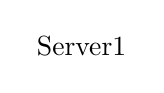
\begin{tikzpicture}[node distance=4cm]
	\node (S1){\server{Server1}};
	\end{tikzpicture}
\caption{Single Server}
\end{figure}

\begin{figure}
\centering
	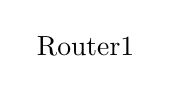
\begin{tikzpicture}[node distance=4cm]
	\node (R1){\router{Router1}};
	\end{tikzpicture}
\caption{Single Router}
\end{figure}

\begin{figure}
\centering\resizebox{\textwidth}{!}{
	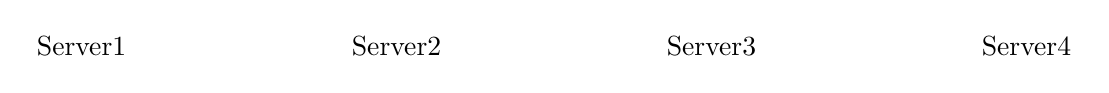
\begin{tikzpicture}[node distance=4cm]
	\node (S1){\server{Server1}};
	\node[right of=S1] (S2){\server{Server2}};
	\node[right of=S2] (S3){\server{Server3}};
	\node[right of=S3] (S4){\server{Server4}};
	\end{tikzpicture}
}
\caption{3 Servers}
\end{figure}

\begin{figure}
\centering\resizebox{\textwidth}{!}{
	\begin{tikzpicture}[node distance=6cm]
	\node (S1){\server{Server1}};
	\node[right of=S1] (R1){\router{Router1}};
	\node[right of=R1] (S2){\server{Server2}};
	\end{tikzpicture}
}
\caption{2 Servers + 1 Router}
\end{figure}

\begin{figure}
\centering\resizebox{\textwidth}{!}{
	\begin{tikzpicture}[node distance=6cm]
	\node (S1){\server{Server1}};
	\node[right of=S1] (R1){\router{Router1}};
	\node[right of=R1] (S2){\server{Server2}};
	\draw[thick] (S1) -- node[ethernet, at start]{eth0} node[ethernet, at end] {ens3f0} (R1) node[speed, midway] {100 Mbps};
	\draw[thick] (R1) -- node[ethernet, at start]{ens3f1} node[ethernet, at end] {eth0} (S2) node[speed, midway] {100 Mbps};
	\end{tikzpicture}
}
\caption{Single Topology}
\end{figure}

\begin{figure}
\centering\resizebox{\textwidth}{!}{
	\begin{tikzpicture}[node distance=4cm]
		\node (S1){\server{Sender}};
		\node[right of=S1] (R1){\router{Router1}};
		\node[right of=S1] (R1){\router{Router1}[true]};
		\node[right of=R1] (R2){\router{Router2}};
		\node[right of=R2] (S2){\server{Receiver}};
		\node[yshift=3.5cm] at ($ (R1) !.5! (R2) $)  (R3) {\router{Router 3}};
		\draw[thick] (S1) -- node[ethernet, at start]{eth0} node[ethernet, at end] {eth0} (R1) node[speed, midway] {100 Mbps};
		\draw[thick] (R1) -- node[ethernet, at start]{eth1} node[ethernet, at end] {eth1} (R2) node[speed, midway] {100 Mbps};
		\draw[thick] (R1) -- node[ethernet, at start]{eth2} node[ethernet, at end] {eth0} (R3) node[speed, midway] {100 Mbps};
		\draw[thick] (R2) -- node[ethernet, at start]{eth2} node[ethernet, at end] {eth1} (R3) node[speed, midway] {100 Mbps};
		\draw[thick] (R2) -- node[ethernet, at start]{eth0} node[ethernet, at end] {eth0} (S2) node[speed, midway] {100 Mbps};
	\end{tikzpicture}
}
\caption{Complicated Topology}
\end{figure}

\end{document}